% This is now Chapter 3
This section outlines the research design, data collection methods, and analytical techniques employed in this comparative study of teacher evaluation approaches.

\subsection{Research Design and Approach}
This study employs a mixed-methods comparative design to evaluate traditional student feedback and multimodal evaluation systems. The research follows a parallel convergent approach where both evaluation methods are applied simultaneously to the same teaching instances, allowing for direct comparison while minimizing contextual variations.
The study will be conducted in a real-world classroom setting, focusing on higher education institutions. The multimodal evaluation system will be implemented in a controlled environment, ensuring that both student feedback and multimodal data are collected under similar conditions. This design allows for a comprehensive analysis of the strengths and weaknesses of each evaluation method.
The research will utilize a combination of quantitative and qualitative data collection methods, including standardized surveys, audio-visual recordings, and discourse analysis \cite{dmello2012multimodal, ochoa2016multimodal}. The quantitative data will be analyzed using statistical techniques to identify correlations and patterns, while qualitative data will undergo thematic analysis to extract meaningful insights.
The study will also incorporate a longitudinal component, allowing for the examination of changes in teaching effectiveness over time. By collecting data at multiple points throughout the semester, the research aims to capture the dynamic nature of teaching and learning processes.

The primary research questions guiding this study are:

\begin{enumerate}
    \item To what extent do multimodal evaluations correlate with traditional student feedback?
    \item Which aspects of teaching effectiveness are captured more accurately by each evaluation method?
    \item How can multimodal systems complement student feedback to provide a more comprehensive evaluation?
    \item What are the practical implications of incorporating multimodal evaluations in institutional assessment frameworks?
\end{enumerate}

\begin{table}[H]
    \normalsize
    \centering
    \caption{ Participant Distribution Across Disciplines and Experience Levels}
    \label{tab:participants}
    \begin{tabular}{lccc}
        \toprule
        \textbf{Discipline} & \textbf{Novice} & \textbf{Experienced} & \textbf{Expert} \\
        \midrule
        STEM & 4 & 4 & 2 \\
        Humanities & 4 & 4 & 2 \\
        Social Sciences & 4 & 4 & 2 \\
        \bottomrule
    \end{tabular}
\end{table}

\subsection{Participants and Sampling}
The study will employ purposive sampling to select 30 instructors from diverse academic disciplines. The inclusion criteria prioritize representativeness across teaching experience (novice to expert), course level (undergraduate and graduate), and subject area (STEM, humanities, and social sciences). Each instructor will be evaluated during 3 different teaching sessions, generating a total of 90 distinct teaching instances for analysis.


Student evaluators will include all enrolled students in the selected course sections, with an estimated total of 1,200-1,500 student participants. Demographic information will be collected from both instructors and students to examine potential correlation patterns and biases.

\subsection{Data Collection Methods}

\subsubsection{Student Feedback Instruments}
Traditional evaluation data will be collected using two complementary instruments:

\begin{itemize}
    \item A standardized quantitative evaluation form using a 5-point Likert scale covering seven dimensions of teaching effectiveness (clarity, organization, engagement, assessment, feedback, accessibility, and overall effectiveness)
    \item Open-ended qualitative questions eliciting specific comments on teaching strengths, areas for improvement, and notable classroom experiences
\end{itemize}

\subsubsection{Multimodal System Components}
The multimodal evaluation system integrates data from three primary sources, as illustrated in Figure \ref{fig:multimodal_components}:

\begin{figure}[H]
    \centering
    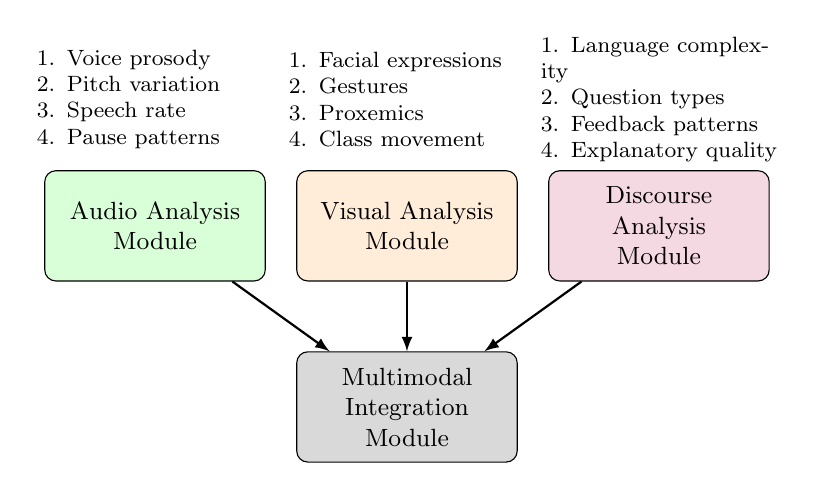
\begin{tikzpicture}[
        module/.style={rectangle, draw, rounded corners, minimum width=2.8cm, minimum height=1.4cm, text width=2.2cm, align=center, font=\small},
        arrow/.style={->, thick, >=latex}
    ]
        % Central component
        \node[module, fill=gray!30] (central) at (0,0) {Multimodal Integration Module};
        
        % Source modules (spaced further apart)
        \node[module, fill=green!15] (audio) at (-3.2,2.3) {Audio Analysis Module};
        \node[module, fill=orange!15] (visual) at (0,2.3) {Visual Analysis Module};
        \node[module, fill=purple!15] (text) at (3.2,2.3) {Discourse Analysis Module};
        
        % Connect modules
        \draw[arrow] (audio) -- (central);
        \draw[arrow] (visual) -- (central);
        \draw[arrow] (text) -- (central);
        
        % Features for each module (moved above and spaced)
        \node[text width=3.0cm, align=left, font=\footnotesize, yshift=0.9cm] at (audio.north) {1. Voice prosody\\2. Pitch variation\\3. Speech rate\\4. Pause patterns};
        \node[text width=3.0cm, align=left, font=\footnotesize, yshift=0.9cm] at (visual.north) {1. Facial expressions\\2. Gestures\\3. Proxemics\\4. Class movement};
        \node[text width=3.0cm, align=left, font=\footnotesize, yshift=0.9cm] at (text.north) {1. Language complexity\\2. Question types\\3. Feedback patterns\\4. Explanatory quality};
    \end{tikzpicture}
    \centering
    \caption{\centering Multimodal system components and feature extraction modules.}
    \label{fig:multimodal_components}
\end{figure}

\begin{enumerate}
    \item \textbf{Audio Module:} Captures speech dynamics using directional microphones positioned strategically in the classroom. The system extracts features related to vocal variety, speech clarity, and emotional tone.
    
    \item \textbf{Visual Module:} Employs two wide-angle cameras (front and rear) to capture teacher movements, gestures, and interactions with students. A deep learning-based pose estimation algorithm tracks key behavioral indicators.
    
    \item \textbf{Discourse Module:} Applies NLP techniques to analyze transcribed classroom dialogue, identifying patterns of instruction, questioning techniques, and feedback quality.
\end{enumerate}

Data collection will occur simultaneously for both evaluation methods during the same teaching sessions to ensure valid comparisons.

\subsection{Data Processing and Feature Extraction}

\subsubsection{Audio Data Processing}
Audio data will be processed to extract the following features:
\begin{itemize}
    \item Prosodic features (pitch, intensity, and speech rate)
    \item Voice quality parameters (jitter, shimmer, and harmonic-to-noise ratio)
    \item Temporal features (speaking time, pause duration, and turn-taking patterns)
    \item Emotion indicators (valence and arousal levels)
\end{itemize}

Audio processing will employ the PRAAT acoustic analysis software with custom scripts for feature extraction, followed by normalization to account for individual voice characteristics.

\subsubsection{Visual Data Analysis}
Visual analysis will focus on extracting behavioral indicators using the following pipeline:

\begin{figure}[t]
    \centering
    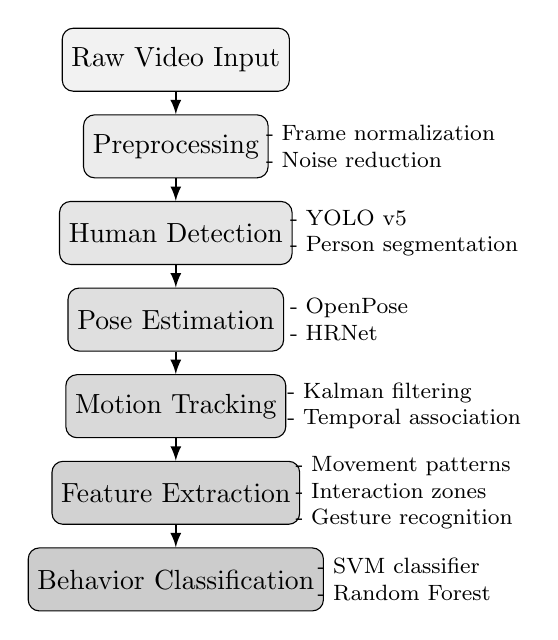
\begin{tikzpicture}[
        stage/.style={rectangle, draw, rounded corners, minimum width=1.8cm, minimum height=0.8cm, align=center, font=\normalsize},
        arrow/.style={->, thick, >=latex}
    ]
        % Processing stages
        \node[stage, fill=gray!10] (input) at (0,0) {Raw Video Input};
        \node[stage, fill=gray!15] (preproc) at (0,-1.1) {Preprocessing};
        \node[stage, fill=gray!20] (detect) at (0,-2.2) {Human Detection};
        \node[stage, fill=gray!25] (pose) at (0,-3.3) {Pose Estimation};
        \node[stage, fill=gray!30] (track) at (0,-4.4) {Motion Tracking};
        \node[stage, fill=gray!35] (extract) at (0,-5.5) {Feature Extraction};
        \node[stage, fill=gray!40] (classify) at (0,-6.6) {Behavior Classification};
        
        % Connect stages
        \draw[arrow] (input) -- (preproc);
        \draw[arrow] (preproc) -- (detect);
        \draw[arrow] (detect) -- (pose);
        \draw[arrow] (pose) -- (track);
        \draw[arrow] (track) -- (extract);
        \draw[arrow] (extract) -- (classify);
        
        % Key techniques
        \node[font=\footnotesize, align=left] at (2.6,-1.1) {- Frame normalization\\- Noise reduction};
        \node[font=\footnotesize, align=left] at (2.9,-2.2) {- YOLO v5\\- Person segmentation};
        \node[font=\footnotesize, align=left] at (2.2,-3.3) {- OpenPose\\- HRNet};
        \node[font=\footnotesize, align=left] at (2.9,-4.4) {- Kalman filtering\\- Temporal association};
        \node[font=\footnotesize, align=left] at (2.9,-5.5) {- Movement patterns\\- Interaction zones\\- Gesture recognition};
        \node[font=\footnotesize, align=left] at (2.9,-6.6) {- SVM classifier\\- Random Forest};
    \end{tikzpicture}
    \caption{ Visual data processing pipeline for teacher behavior analysis.}
    \label{fig:vision_pipeline}
\end{figure}

The system will quantify spatial classroom dynamics, including:
\begin{itemize}
    \item Classroom coverage (percentage of classroom space utilized)
    \item Proximity patterns (time spent in different classroom zones)
    \item Student interaction frequency (number and distribution of individual engagements)
    \item Gesture frequency and type (emphatic, illustrative, and regulatory)
\end{itemize}

\subsubsection{Linguistic and Discourse Analysis}
Classroom dialogue will be transcribed automatically using speech-to-text technology and analyzed for:
\begin{itemize}
    \item Question complexity (based on Bloom's taxonomy)
    \item Wait time after questions
    \item Feedback patterns (evaluative, corrective, or elaborative)
    \item Language complexity (lexical diversity and sentence structure)
    \item Instructional clarity indicators (use of examples, analogies, and summaries)
\end{itemize}

\subsubsection{Student Feedback Processing}
Quantitative feedback will be analyzed using descriptive and inferential statistics, while qualitative comments will undergo thematic analysis using a dual-coding approach to identify emergent patterns. NLP techniques will also be applied to extract sentiment and topical focus from written comments.

\subsection{Evaluation Metrics}
The comparative analysis will employ the following metrics to assess the relationship between traditional and multimodal evaluations:

\begin{table}[t]
    \centering
    \normalsize
    \caption{Evaluation Dimensions and Corresponding Metrics}
    \label{tab:metrics}
    \begin{tabular}{lcc}
        \toprule
        \textbf{Dimension} & \textbf{Student Feedback Metric} & \textbf{Multimodal Metric} \\
        \midrule
        Engagement & Likert rating (1-5) & Interaction frequency + \\
         & & Voice animation index \\
        \midrule
        Clarity & Likert rating (1-5) & Speech rate + Pause ratio + \\
         & & Example frequency \\
        \midrule
        Organization & Likert rating (1-5) & Topic coherence score + \\
         & & Transition clarity index \\
        \midrule
        Responsiveness & Likert rating (1-5) & Response time + \\
         & & Student engagement rate \\
        \bottomrule
    \end{tabular}
\end{table}

Statistical analyses will include:
\begin{itemize}
    \item Correlation analysis between student ratings and multimodal metrics
    \item Factor analysis to identify underlying constructs across evaluation methods
    \item Multiple regression to predict student satisfaction from multimodal features
    \item Paired comparisons to identify systematic differences between methods
\end{itemize}

\subsection{Ethical Considerations}
This research has received approval from the Institutional Review Board (IRB) and implements the following ethical safeguards:
\begin{itemize}
    \item Informed consent from all participating instructors and students
    \item Data anonymization protocols for both traditional and multimodal datasets
    \item Secure data storage with encryption and access controls
    \item Options for participants to review their data and withdraw at any time
    \item Transparent communication about data usage and research findings
\end{itemize}

All classroom recordings will be processed on secure, local servers rather than cloud-based solutions to enhance privacy protection. Face-blurring technology will be applied to student images in accordance with privacy regulations.
